\section{Mapzen & QGIS}
Mapzen Merupakan laboratorium pemetaan open source dibawah Samsung Accelatoryang membangun dan mendukung data dan software terbuka untuk mempromosikan ekosistem pemetaan yang sehat. Tim Pengembangan dari Mapzen merupakan salah satu divisi dari SRA (Samsung Research Amerika) yang berfokus pada komponen inti dari platform geo, termasuk pencarian, rendering, navigasi, dan data.

Aplikasi Mapzen memakai data dan software lisensi dari OpenStreetMap. Jadi apabila Anda memakai aplikasi Mapzen harus mempunyai account di OpenStreetMap. Aplikasi Mapzen dibangun berdasarkan project open source OpenScienceMap, Pelias, Open Source Routing Machine (OSRM, dan SDK open source dari Mapzen, dapat mengakses hardware GPS di perangkat mobile untuk fitur navigasi dan peta pada saat berjalan, mengendarai mobil maupun bersepeda.

Keunggulan dari produk Mapzen adalah penggunaan mesin rendering fleksibel yang disebut juga Tangram yang digunakan untuk menampilkan peta digital dalam nuansa 2D maupun 3D secara real-time. Mapzen dibangun dari berbagai peralatan open-source yang dikemas ke dalam layanan Web dan di hosting di server Mapzen.

Beberapa fitur  dari Mapzen yaitu:
\item Tangram, sebuah mesin pemetaan fleksibel yang dirancang sebagai rendering peta 2D dan 3D secara real-time.
\item Valhalla, sebuah layanan routing open-source dari Mapzen sebagai aplikasi routing di sisi client dan solusi host.
\item Metro Extracts, porsi berukuran kota dari database OpenStreetMap, yang disajikan secara mingguan.
\item Pelias, modular open source geocoder menggunakan ElasticSearch sebagai fast autocomplete dan forward & reverse geocoding.

\subsection{Sejarah Mapzen}
Pada akhir 2007, Simon Willison meluncurkan beberapa situs web yang paling berguna di internet. Situs web itu disebut Get Lat Lon dan keseluruhan tujuannya adalah untuk memungkinkan pengunjung menemukan garis lintang dan bujur sebuah titik di peta.
Situs web ini dibangun menggunakan Google Maps API dan memiliki formulir untuk alamat geocoding atau nama tempat namun antarmuka utama adalah peta sederhana dengan satu set garis bidik yang berpusat di area pandang. Lat Lat hanya akan mencetak koordinat geografis dari lokasi mana pun yang berada di bawah garis bidik. Cemerlang!
Di suatu tempat antara tahun 2007 dan sekarang perpanjangan domain untuk Get Lat Lon terjerumus dan sekarang ini ... sesuatu yang lain sama sekali, sesuatu yang tidak berharga untuk dipertautkan. Anda masih bisa merasakan kesederhanaan dan keanggunan keseluruhan desainnya karena ada snapshot dari situs web di Mesin Wayback kecuali ... tidak ada karya Javascript lagi.
Pada tahun 2009 saya memutuskan untuk menulis versi saya sendiri dari Get Lat Lon. Alih-alih menggunakan Google Maps API, itu akan menggunakan semua perangkat lunak dan data yang terbuka. Data peta akan dari OpenStreetMap. Ubin peta berasal dari CloudMade dengan menggunakan kartografi baru yang menarik dari Stamen Design. Ini akan menggunakan perpustakaan modestmaps.js untuk mengelola semua ubin tersebut. Ini akan mendukung API Geolocation berbasis-yang saat ini masih ada untuk membantu menentukan lokasi Anda. Geocoding akan ditangani oleh Flickr dan selain geocoding juga akan mencoba membalikkan geocode lokasi Anda dan menampilkan bentuk tempat yang dikandung oleh latlon, sekali lagi menggunakan 
Dan ... itu akan sangat pintar dan modular sehingga bisa mendukung banyak penyedia layanan dan Anda bisa memasukkannya ke halaman web manapun dan itu akan berhasil, seolah seperti sihir. Itu disebut I Am Here dan saya pikir saya satu-satunya orang yang pernah menggunakannya tapi masih berjalan. Pada tahun 2014, CloudMade keluar dari bisnis genteng dan secara harfiah tidak banyak yang bisa dilihat lagi.
Saya cukup yakin bahwa itu persis satu baris kode untuk menentukan penyedia peta baru agar saya Disini bekerja lagi tapi jujur saja hanya melihat semua kode terlalu-terlalu pintar sekarang, pada tahun 2016, melelahkan. Juga, lihat bagaimana informasi perizinan pada data peta belum diperbarui untuk mencerminkan peralihan ke ODbL ...
Maju cepat ke tahun lalu (2015) dan pekerjaan telah dimulai dengan sungguh-sungguh di gazetteer Who's On First (WOF) di Mapzen. Sebagian dari pekerjaan itu adalah membangun hierarki untuk setiap rekaman di dalam gazetteer yang merupakan masalah ayam dan telur. Kami telah mengotomatisasi proses ini dengan tool general purpose point-in-polygon yang telah kami tulis secara in-house dengan menggunakan bahasa pemrograman Go.

\subsection{Menu Pada QGIS}
source type ini berupa pilihan :
File | Directory | Database | Protocol
Protocol yang disupport adalah URI (Uniform Resources Identifier) untuk GeoJSON, GeoJSON sendiri merupakan enkoding open format data geografis bertipe JavaScript Open Notation.
Database yang disupport antara lain ESRI Personal Geodatabase, ODBC, Postgre, dan MySQL, artinya anda bahkan bisa buka Geodatabase ESRI walaupun kemungkinan ada beberapa format data khusus yang hilang, tetapi spatial-nya akan tetap dapat terbaca.

\subsection{Tambahkan shapefile OSM2PGSQL ke QGIS}
Cara menambahkan shapfile OSM2PGSQL ke QGIS:
\begin{enumerate}
\item Jalankan QGIS dan tampilkan peta kosong.
\item Pada panel Browser, navigasikan ke folder dimana shapefile disimpan dan buka file 'bandung_indonesia.osm2pgsql-shapefiles'.
\item Perhatikan bahwa file tersebut berisi tiga shapefile, dinamai dengan tipe geometri: line, point ,dan polygon.
\item Klik dua kali pada layer line untuk membukanya di peta. contoh yang di klik adalah 'bandung_indonesia_osm_line'. \ref{micin1}
\begin{figure}[ht]
	\centerline{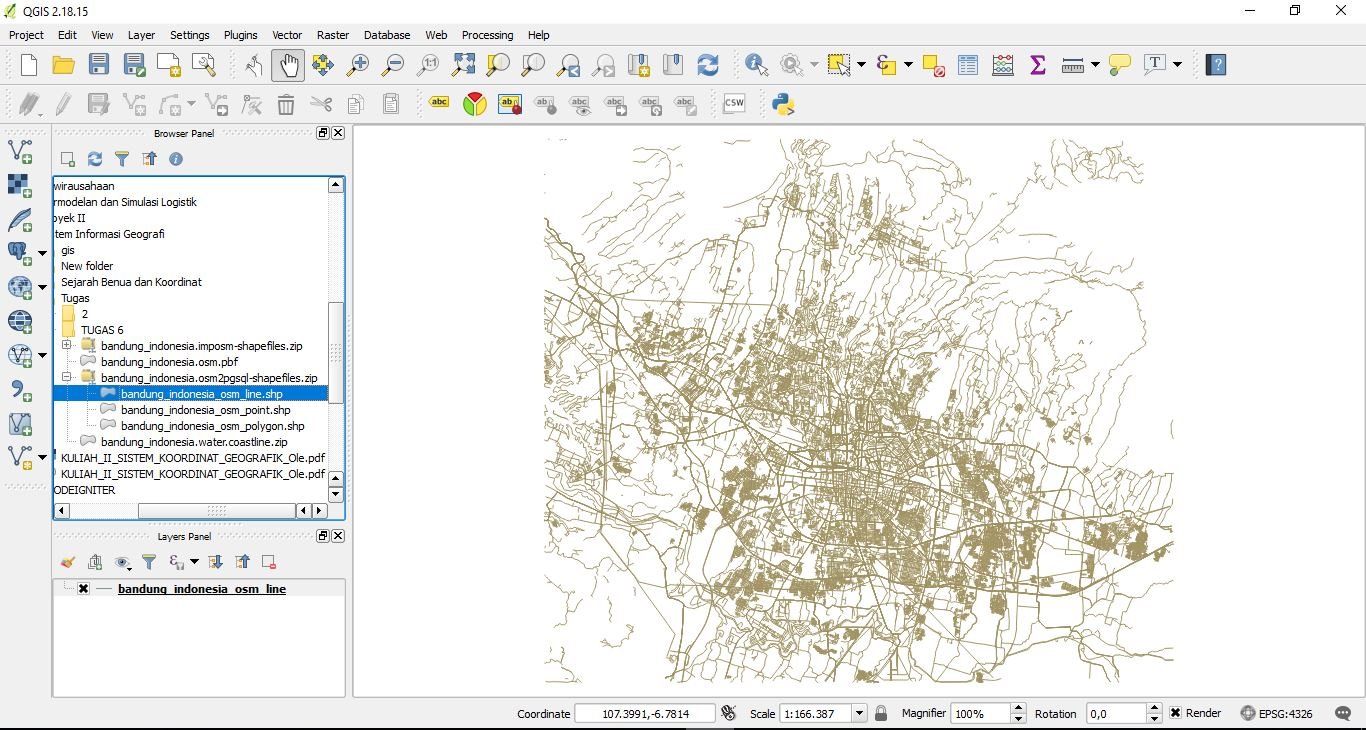
\includegraphics[width=1\textwidth]{figures/micin1.JPG}}
	\caption{OSM2PGSQL ke QGIS}
	\label{micn1}
	\end{figure}
